\documentclass[boxedsections ,landscape, a0]{sciposter_v2}

\usepackage{epsfig}
\usepackage{amsmath}
\usepackage{amssymb}
\usepackage{multicol}
\usepackage{wrapfig}
\usepackage{floatflt}
\usepackage{psfrag}


%colour of the boxes
\definecolor{BoxCol}{RGB}{163,193,173}


\leftlogo[0.15]{graphics/CUnibig}
\rightlogo[0.2]{graphics/logo_siggraph_vancouver}

\conference{{\bf SIGGRAPH 2011}, 38th International Conference and Exhibition on Computer Graphics and Interactive Techniques, 7-11 August 2011, Vancouver, Canada}

\title{\textsc{Simulation of breathing for medical applications}}

\author{Thierry J. Maldonado and Joan Lasenby}

\institute{Signal Processing and Communications Laboratory, Department of Engineering, University of Cambridge}

\email{\{tjm53, jl221\}@cam.ac.uk}

\renewcommand{\titlesize}{\huge}


\begin{document}

\maketitle
\begin{multicols}{4}

%%%%%%%%%%%%%%%%%%%%%%%%%%%%%
%	Introduction
%%%%%%%%%%%%%%%%%%%%%%%%%%%%%
\section*{Introduction}


This work describes further research on the \textbf{Structured Light Plethysmography} (SLP) \cite{2010slp} project which is a non-invasive method for pulmonary function testing using visible light. As the device captures only the front
of the chest wall, \textbf{we cannot infer the absolute volumes of the lungs}
but only volume changes of the thoracic cage. However, when it
comes to examining respiratory function in a patient, absolute volumes
represent a crucial piece of information. 

\begin{wrapfigure}{r}{0.4\columnwidth}

  \begin{center}
  
    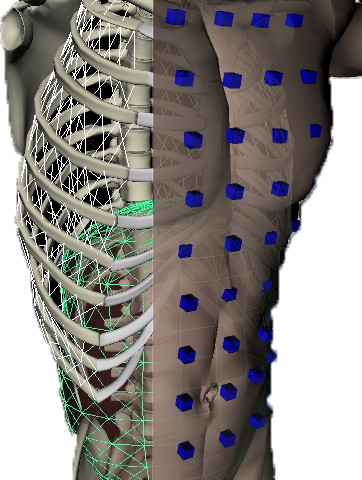
\includegraphics[width=0.4\columnwidth]{imgs/model}
     
  \end{center}
\vspace{-\bigskipamount}     

\end{wrapfigure}

\
\\
\
In order to address
this problem we use \textbf{optimisation techniques} to fit SLP data to a
\textbf{highly detailed 3D model of the human torso} (composed of rigid
parts and muscles) that we have created. Our simulation provides
us with both \textbf{the optimal muscle inputs to simulate breathing} - to
date, these muscle activations have remained mysterious and been
simplified to sine functions in the literature - and \textbf{the absolute volumes
of the lungs} for a given SLP dataset.

\
\\
\
\textbf{Previous attempts have concentrated more on the visual
side} of the simulations than on the medical applications:


\cite{lee2009comprehensive} describes
a model of the whole upper body but with few respiratory muscles
of the rib cage and with no diaphragm, which is an essential muscle
in breathing. 


\cite{zordan2004breathe} uses a skeleton model which lacks anatomical 
realism and simplifies the articular bones
in the spine and the rib cage by grouping and treating them as a
single rigid body. 

\textbf{Our model has high anatomical accuracy}. In addition, it has \textbf{high-level controls}, is \textbf{fully
tunable} (each muscle can be activated independently) and \textbf{can be
fitted to different patient anatomies}.



%%%%%%%%%%%%%%%%%%%%%%%%%%%%%
%	Breathing mechanisms
%%%%%%%%%%%%%%%%%%%%%%%%%%%%%
\section{Breathing mechanisms}


\begin{wrapfigure}{l}{0.45\columnwidth}
\vspace{-\bigskipamount}     
  \begin{center}
    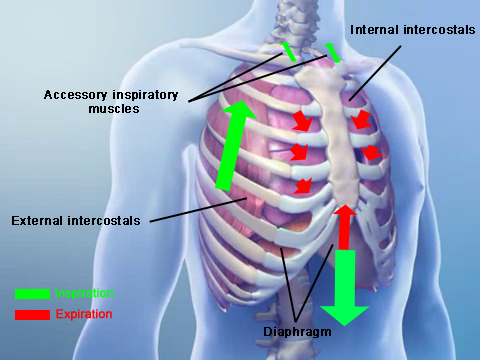
\includegraphics[width=0.5\columnwidth]{imgs/respiratory_schema}
      \emph{Respiratory system.}
  \end{center}
     
\end{wrapfigure}

Breathing entails expanding (inspiration) and contracting (expiration)
the chest wall. From a physiological point of view, this is done
through two different moving parts of the body: the rib cage and the
abdominal cavity. The rib cage is driven by three types of muscles: the scalene muscles and the external intercostals which expand the
rib cage by lifting up the ribs and the internal intercostals which
move the rib cage down. The abdominal cavity is put into motion
by the diaphragm, which contributes to the expansion of lung volume
by pushing down the organs inside the abdominal cavity resulting
in the ventral abdominal wall moving outwards, and the abdominal
muscles, which push the ventral abdominal wall inwards.


%%%%%%%%%%%%%%%%%%%%%%%%%%%%%
%	Structured Light Plethysmography
%%%%%%%%%%%%%%%%%%%%%%%%%%%%%

\section{Structured Light Plethysmography}

Structured Light Plethysmography is a non-invasive method for pulmonary function
testing using visible light. This technique uses two motion capture cameras and a
known grid which is projected onto the chest and abdomen of a patient.

%\vspace{-\bigskipamount}   

\begin{figure}

\subfigure[\emph{Diagram of the SLP device.}]{
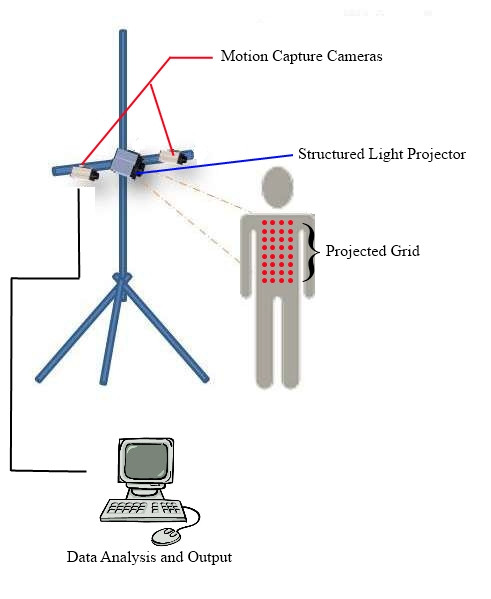
\includegraphics[width=0.4\columnwidth]{imgs/slp_device}
}
\subfigure[\emph{SLP in action.}]{
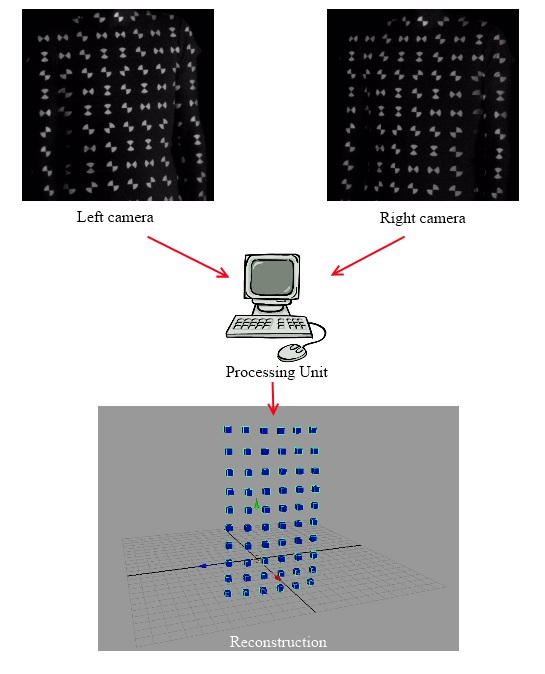
\includegraphics[width=0.4\columnwidth]{imgs/slp_reconstruction}
}
\end{figure}

%\vspace{-\bigskipamount}   

It relies on triangulation to reconstruct the space locations of the grid points projected
by combining the images of the two cameras for each frame. 
The SLP system ultimately provides us with the space coordinates over time of the grid
points that are located on the chest and abdomen of a patient breathing. From the
25x30-point initial grid, a subset of varying size usually from 5x5 to 10x10 is finally
retained.



%%%%%%%%%%%%%%%%%%%%%%%%%%%%%
%	3D Model
%%%%%%%%%%%%%%%%%%%%%%%%%%%%%
\section{3D Model}


\subsection{Rigid-body Components}


\begin{wrapfigure}{r}{0.3\columnwidth}
\vspace{-2.5\bigskipamount}
  \begin{center}
    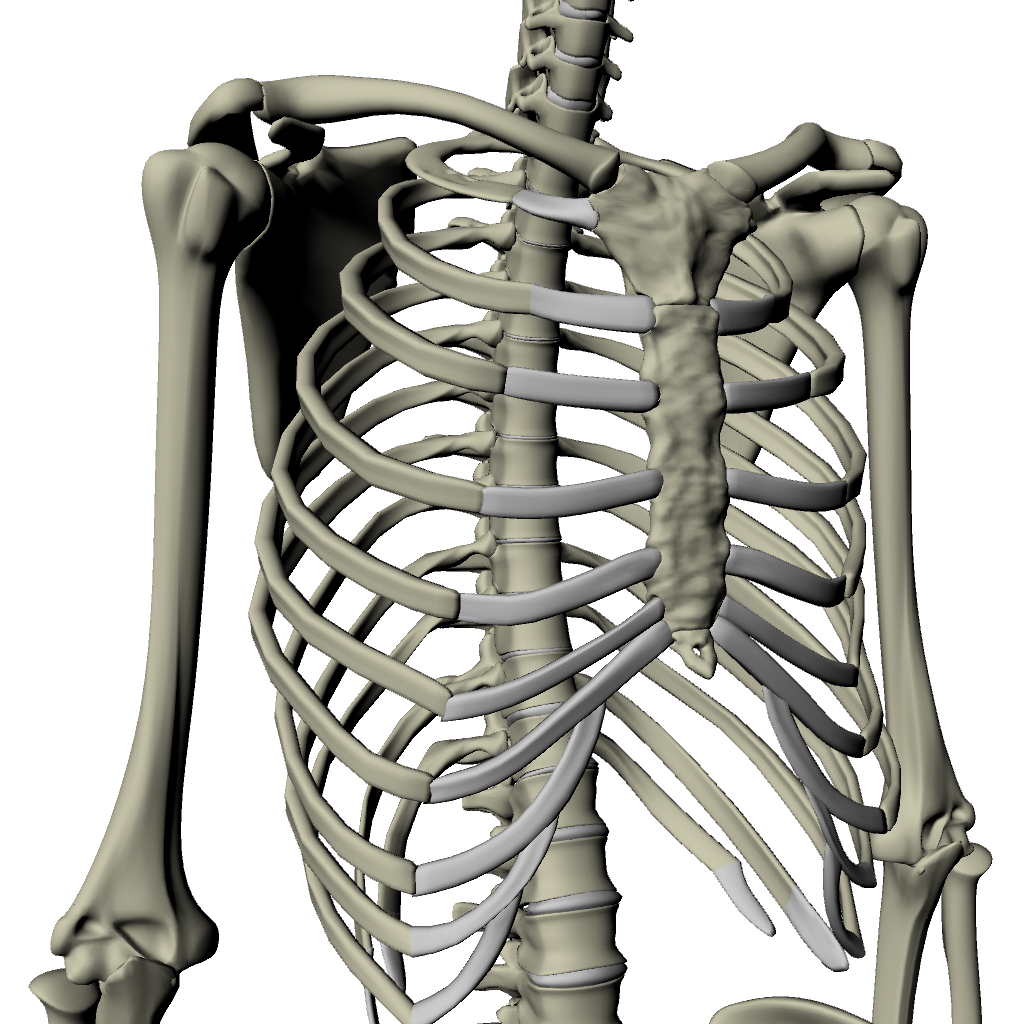
\includegraphics[width=0.3\columnwidth]{imgs/skeleton}
     \emph{Skeleton model.}
     
  \end{center}
  \vspace{-\bigskipamount}
 \end{wrapfigure}


As the model serves medical purposes, it must have high anatomical accuracy in both the dimensions of the rigid parts and the locations and the types of joints linking them. 
We used as sources several anatomy books.

\vspace{0.5\bigskipamount}

\subsection{Spring Muscle Element}
We modelled each muscle we used as a spring and a damper in parallel linking \emph{nodal masses} which are in our case the different bones. The spring $ S_{ij} $, which connects node $ i $ to neighbouring nodes $ j $, exerts the force $ \mathbf{f}_{ij}^s $ on node $ i $ and $ - \mathbf{f}_{ij}^s $ on node $ j $:

\begin{equation} \label{eq:spring_muscle} \mathbf{f}_{ij}^s = -( c_{ij} e_{ij} + \gamma_{ij} \dot{e}_{ij} ) \frac{\mathbf{r}_{ij}}{\lVert \mathbf{r}_{ij} \rVert} \end{equation}

where $ c_{ij} $ is the stiffness gain, $ \gamma_{ij} $ is the damping gain and $ e_{ij}(t) = \lVert \mathbf{r}_{ij} \rVert - l_{ij} $ is the deformation of the spring with separation vector $ \mathbf{r}_{ij}(t) = \mathbf{x}_{j} - \mathbf{x}_{i} $. The rest length of the spring is $ l_{ij} $.

The different parameters (stiffness and damping gain) were tuned individually
depending on the type of muscle.

\vspace{0.5\bigskipamount}

\subsection{Simulation of the Respiratory Muscles}
\vspace{-1.5\bigskipamount}
	\subsubsection{Rib cage}
\vspace{-0.5\bigskipamount}
Between each rib, twelve to fourteen spring elements were
attached to simulate the external (green) and the internal (red) intercostal muscles. To model each intercostal layer, 250 spring muscle elements were used. We modelled the scalene muscles (light blue) with 12 spring elements linking the cervical vertebrae
C6 to the first rib.

\begin{figure}
\centering
\subfigure[\emph{Intercostal muscles.}]{
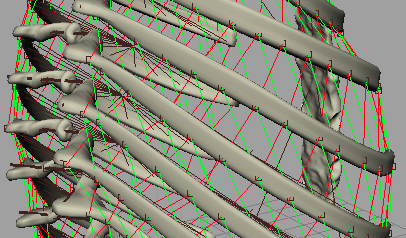
\includegraphics[height=0.3\columnwidth]{imgs/simu_intercostals_zoom}
}
\subfigure[\emph{Scalene muscles.}]{
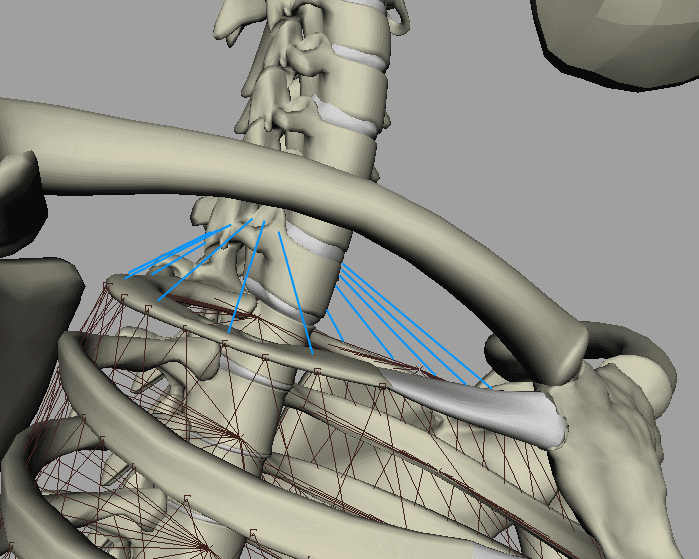
\includegraphics[height=0.3\columnwidth]{imgs/simu_scalenes}
}
\end{figure}	
\vspace{-2\bigskipamount}

	\subsubsection{Abdominal cavity}
	
\begin{wrapfigure}{r}{0.4\columnwidth}
\vspace{-2.5\bigskipamount}
  \begin{center}
    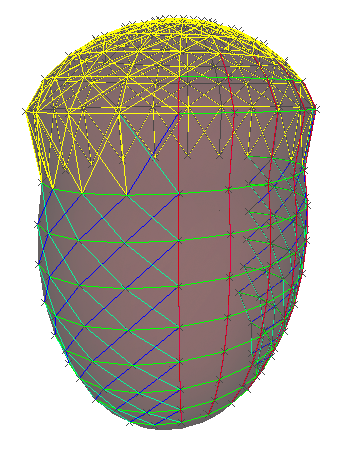
\includegraphics[width=0.4\columnwidth]{imgs/abdo_mus}
    
     \emph{Abdominal muscles.}
  \end{center}
%\vspace{-\bigskipamount}     
\end{wrapfigure}

The diaphragm (yellow) and the four abdominal muscles were also modelled with spring muscles: the transversus abdominis (green), the rectus abdominis (red), the external obliques (light blue) and the internal obliques (dark blue).
\
\\
\

The abdominal compartment can be reasonably considered as fully incompressible (contains between 100 and 300 mL of abdominal gas and the
rest is incompressible). Thus, to model the movement we assume that the pressure $P$ inside the cavity is determined by Hooke's law:

\begin{equation}P \propto \left(\frac{V_{0}}{V} - 1\right) \end{equation}

where $V_{0}$ is the original volume and $V$ the current volume of the abdominal cavity. Since in our model the surface of the cavity is polygonal, being composed of triangles, the volume is calculated as the sum of tetrahedra inside the cavity. In order to make the active vertices of the front of the belly move outwards when the diaphragm contracts, for each active vertex, a force $F_{v}$ proportional to the pressure $P$ times the area $A$ of the triangle attached to the vertex is applied.

\begin{equation}\vec{F_{v}} = P\frac{A}{3}\vec{n} \end{equation}

where $\vec{n}$ is the perpendicular direction to the triangle. The division by 3 accounts for the three vertices composing the triangle.


	
%%%%%%%%%%%%%%%%%%%%%%%%%%%%%
%	Fitting datasets to the model
%%%%%%%%%%%%%%%%%%%%%%%%%%%%%
\section{Fitting datasets to the model}	

\subsection{Skin mesh}
Our skeleton model can be shaped and an adapted skin mesh created with the open source software Make Human \cite{makehuman2010} according to some physiognomy data for the patient such as gender, age, height, weight and  breast size.

  \begin{center}
    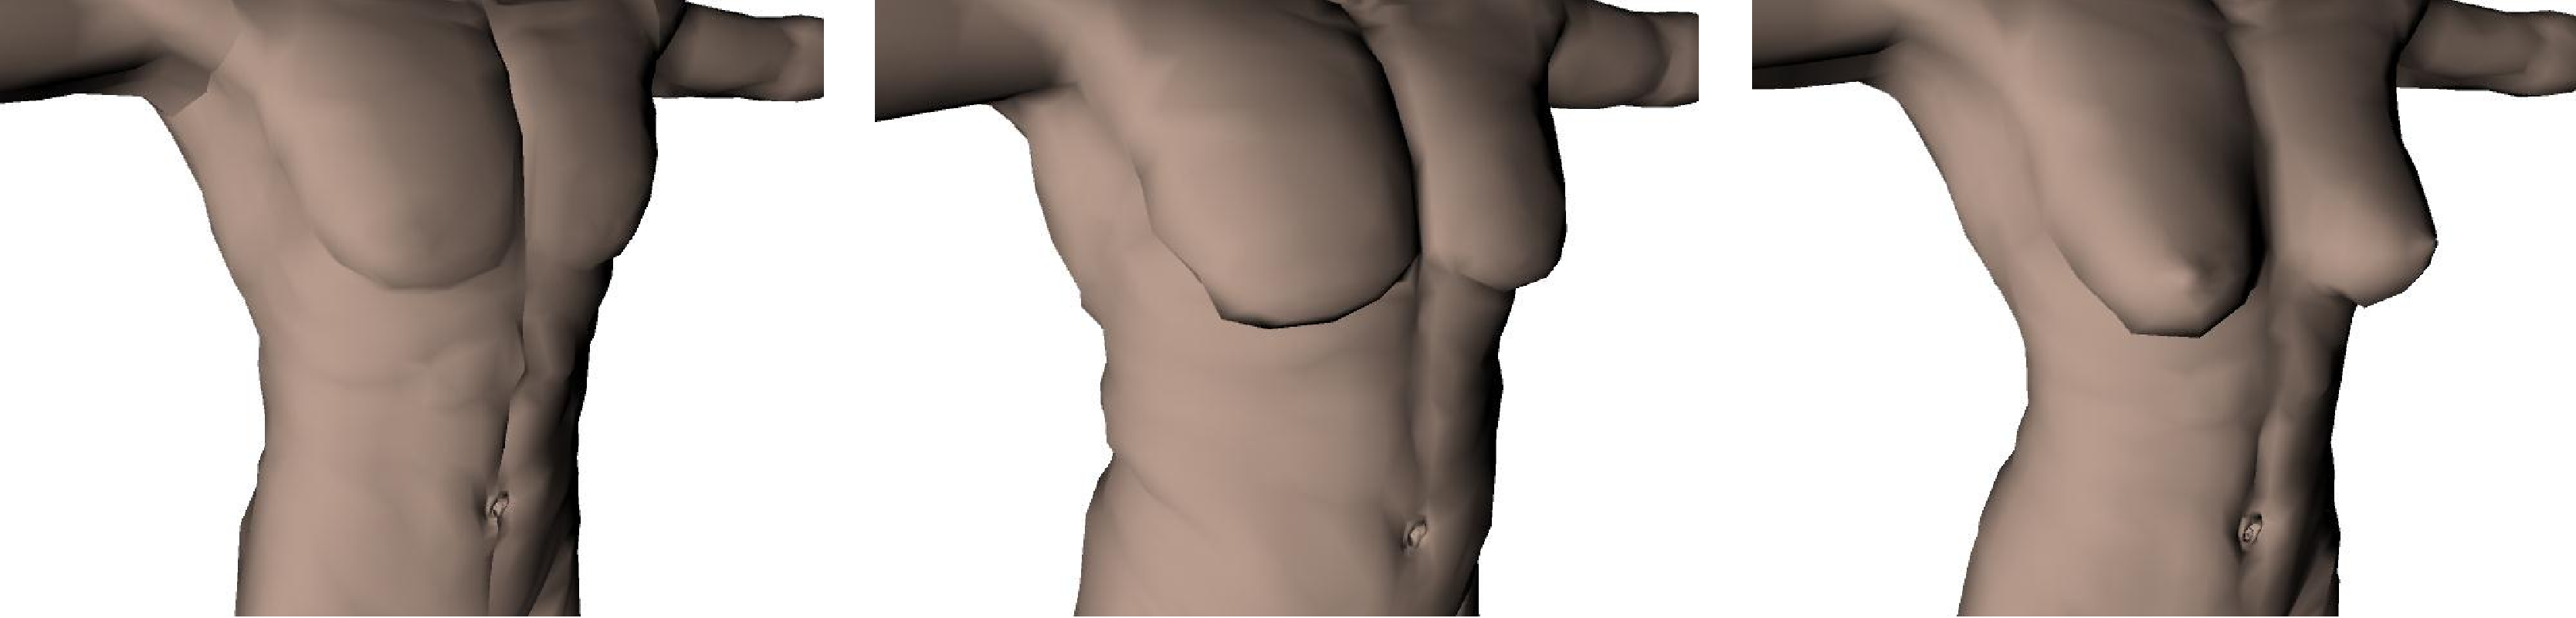
\includegraphics[width=0.85\columnwidth]{imgs/skins}
    
    
     \emph{An adapted skin mesh is created to reduce the fitting error.}     
  \end{center}
%\vspace{-\bigskipamount}     


We compute a normalised error between the skin mesh and the current SLP grid by summing the distances between each grid point and the closest vertex on the skin. We then displace the vertices to the grid point locations they are associated with and then smooth the whole skin to avoid skinning artefacts.

\subsection{Optimisation}

Once the torso model is fitted to a patient anatomy, we use an optimisation technique to fit real datasets from the patient using the output data acquired with the Structured Light Plethysmography technique. 
Currently, we use the Nelder-Mead Downhill
Simplex Method to optimise over several muscle parameters and
we use as cost function the distance error over a whole dataset between
the grid points of the SLP and their closest vertices on the
skin model. 

  \begin{center}
  \vspace{-\bigskipamount}     

    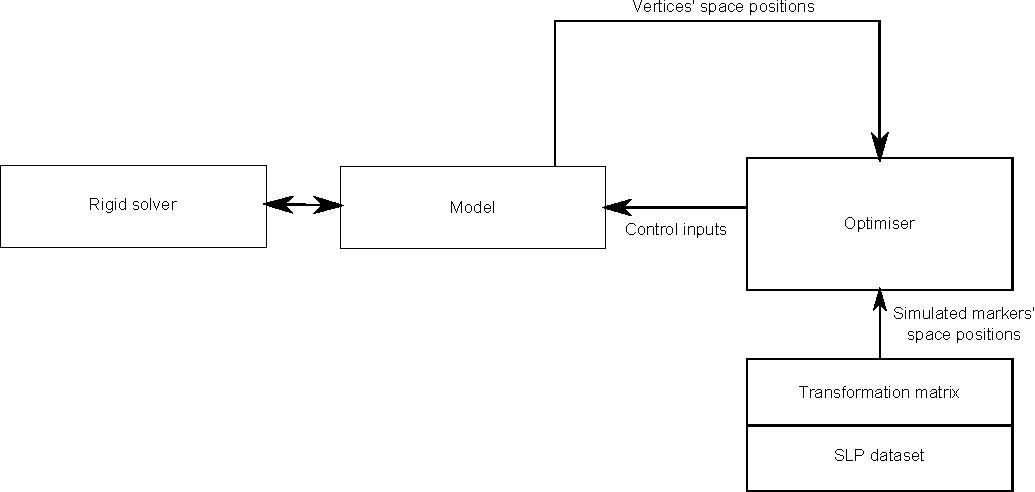
\includegraphics[width=\columnwidth]{imgs/slp_optim}
      \emph{SLP-driven system overview.}

   \vspace{-\bigskipamount}     
  \end{center}
  
%%%%%%%%%%%%%%%%%%%%%%%%%%%%%
%	Fitting datasets to the model
%%%%%%%%%%%%%%%%%%%%%%%%%%%%%
\section*{Results \& Validation}	
Thus, we get the volume of the lungs of our simulation
over time and the different activation muscle parameters that drive
the breathing. We present results which show the visual realism of
the resultant breathing. The validation of our method is done by 
comparing the simulated lung volumes with spirograms. We have used 
statistical methods to compare both the raw time series data and 
the extracted parameters.

\begin{figure}

\centering
\subfigure[\emph{Optimal activations.}]{
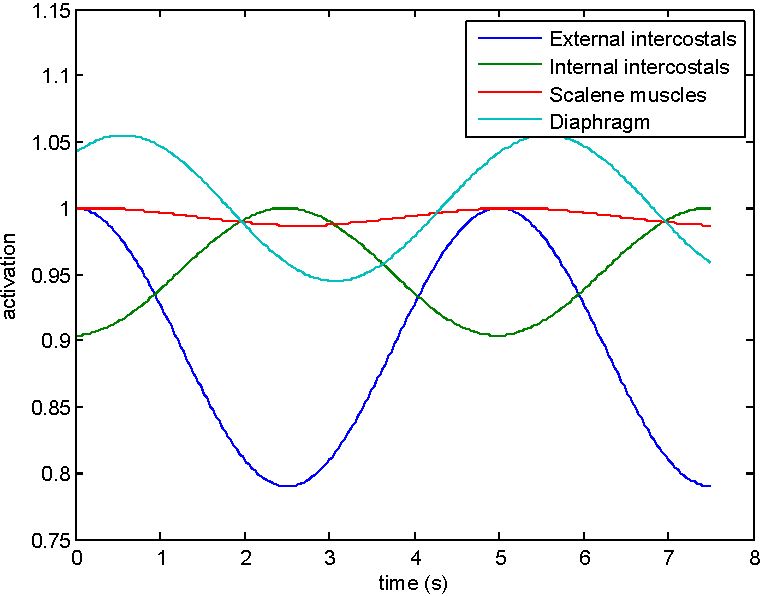
\includegraphics[height=0.35\columnwidth]{imgs/simu_act}
}
\subfigure[\emph{Spirogram vs Simulation.}]{
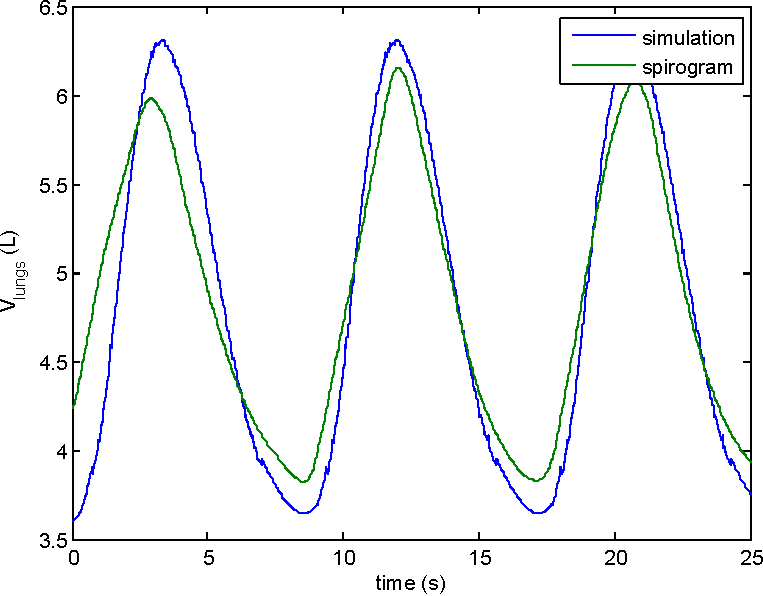
\includegraphics[height=0.35\columnwidth]{imgs/comparaison_spir_simu}
}

\vspace{-\bigskipamount}   
\end{figure}






\small
\nocite{*}
\bibliographystyle{unsrt}
\bibliography{bibliography}



\end{multicols}
\end{document}